\documentclass[12pt, letterpaper]{article}

% Imports
\usepackage{fancyhdr}
\usepackage{geometry}
\usepackage{icomma}
\usepackage{amsmath}
\usepackage{multicol}
\usepackage{mathptmx}
\usepackage{anyfontsize}
\usepackage{t1enc}
\usepackage{tabto}
\usepackage{listings}
\usepackage{filecontents}
\usepackage{subcaption}
\usepackage{tikz}
\usepackage[parfill]{parskip}
\usepackage{graphicx}
\usepackage[]{mdframed}
\usepackage{amsmath}
\usepackage[makeroom]{cancel}
\usepackage{pgfplots}
\usepackage{pgfplotstable}
\usepackage{xfrac}
\usepackage{amssymb}
\usepackage{mathtools}
\pgfplotsset{compat=1.18}
\usetikzlibrary{patterns}
\usepgfplotslibrary{polar}
\usepgfplotslibrary{fillbetween}

\geometry{margin=2.5cm}

\newcommand{\name}{Kaleb Burris}
\newcommand{\classname}{MATH F253, Elizabeth S. Allman, University of Alaska Fairbanks}
\newcommand{\assignment}{FILL IN ASSIGNMENT NAME}

\pagestyle{fancy}

\fancyhead[L]{
    \name 
    \newline
    \classname
    \newline
    \assignment
}

\newcommand{\horizontal}{\noindent\rule{\hsize}{0.4pt}}

\setlength{\headheight}{42pt}
\setlength{\headsep}{0.25in}
\setlength{\columnsep}{0.35cm}
\setlength{\columnseprule}{1pt}

\usepackage[T1]{fontenc}
\usepackage{lmodern}

% Put class number, class name, and professor 
% name.
% Use only in case of emergency, this
% should be covered by the preamble.
% \renewcommand\classname{}

% Put the assignment name with \S if 
% necessary for the section and the question 
% numbers.
\renewcommand\assignment{Lab 2: Energy Transfer, 9/14/2023, Partner: Quency Snow}

\graphicspath{ {./lab02images/} }

\begin{document}
    \section*{Data and Analysis}
    \begin{enumerate}
        \item [1.]\mbox{}
        \begin{mdframed}
            \begin{center}
                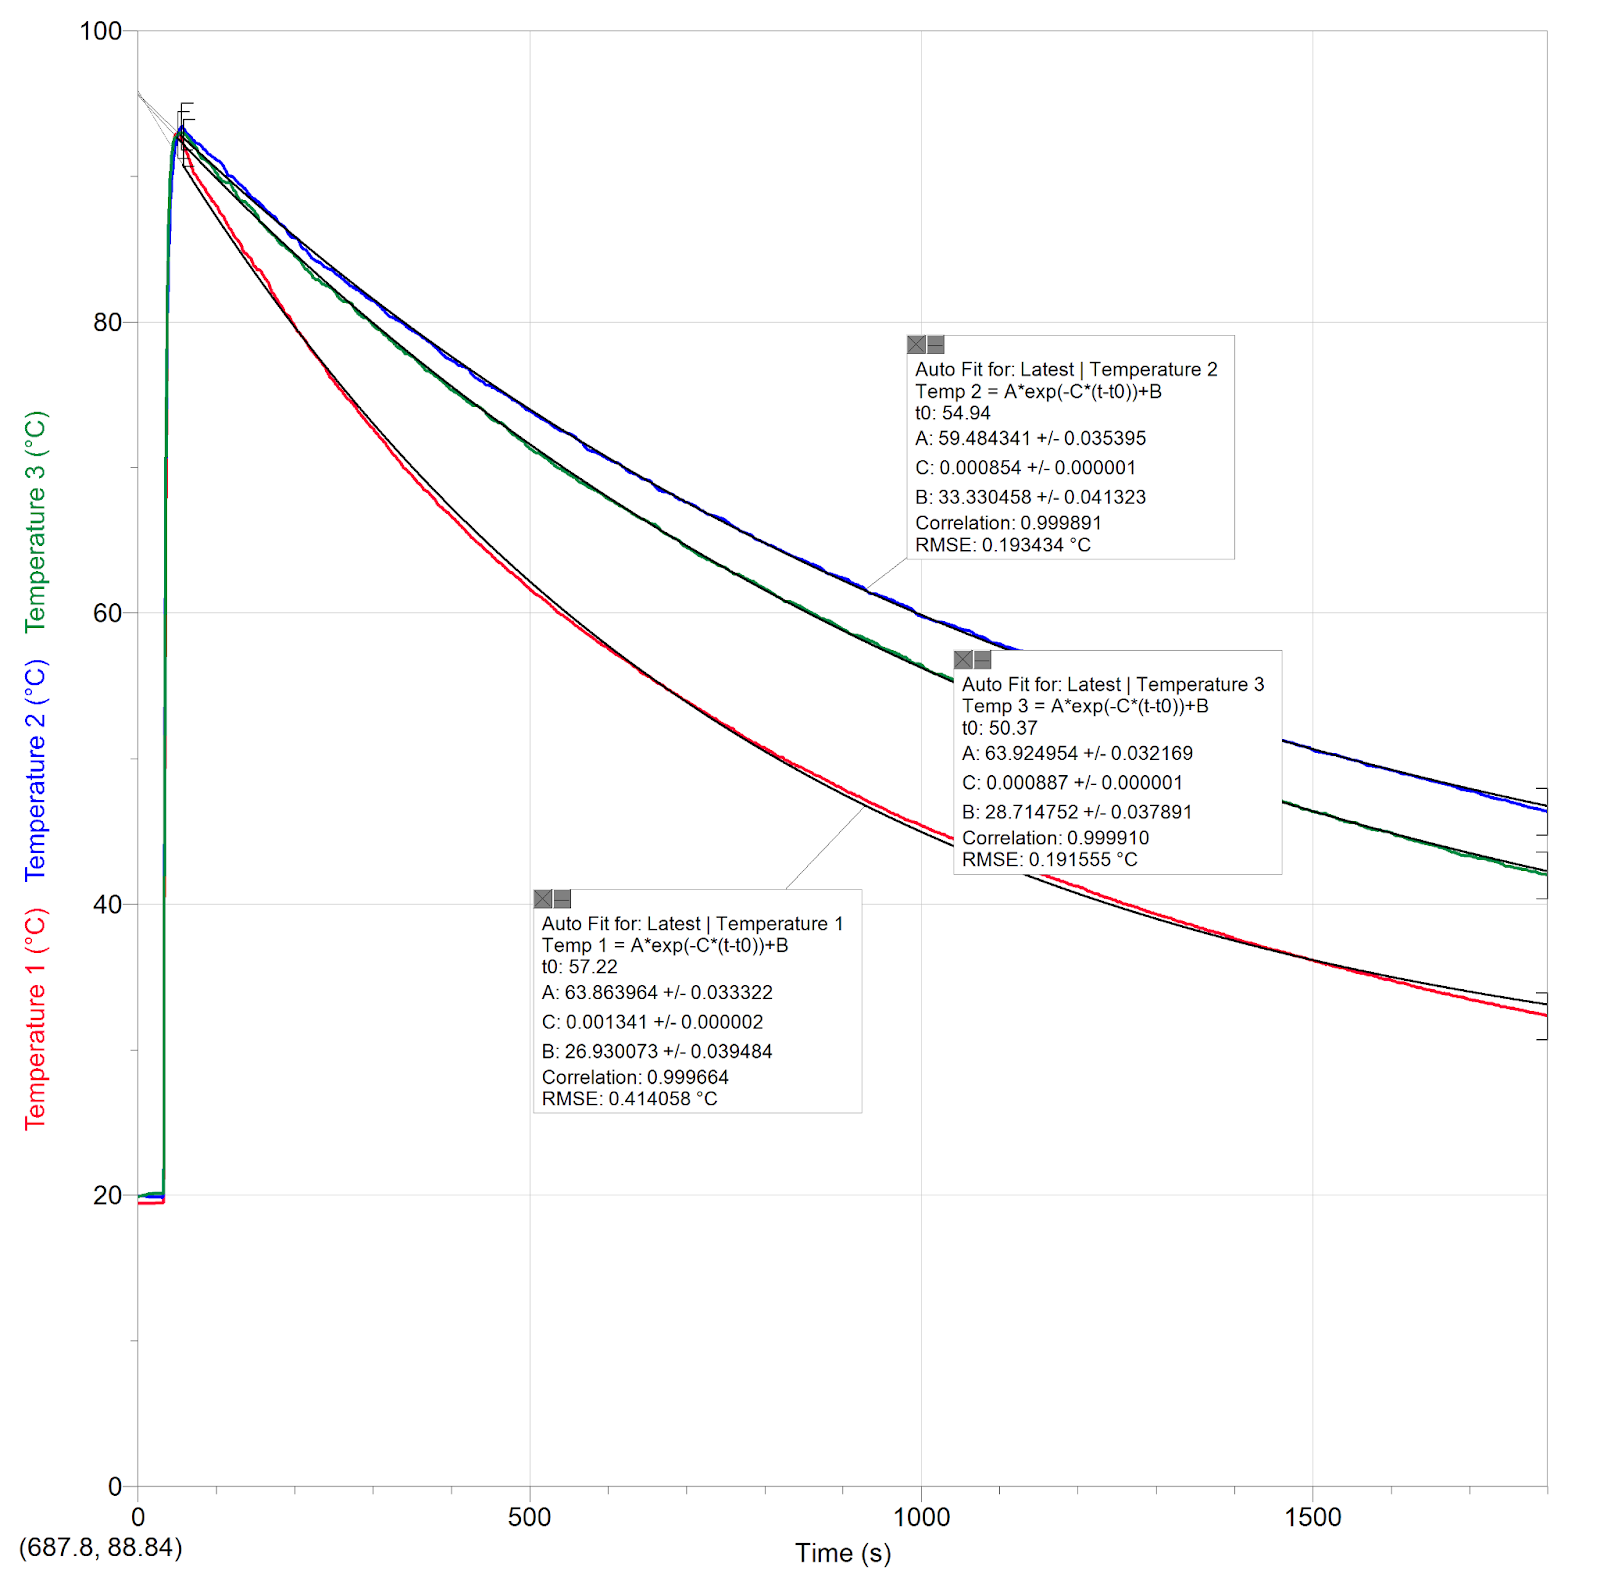
\includegraphics[width=0.4\textwidth]{Untitled.png}
            \end{center}
        \end{mdframed}

        \item [2.]\mbox{}
        \begin{mdframed}
            \begin{center}
                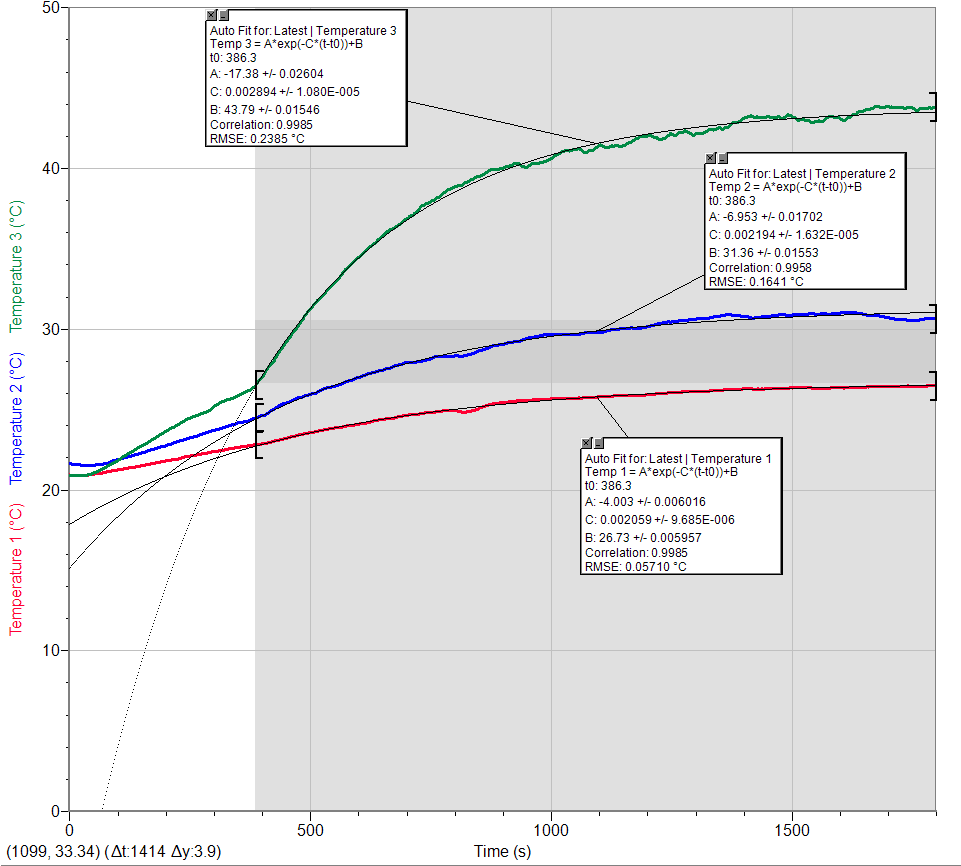
\includegraphics[width=0.4\textwidth]{thermal.png}
            \end{center}
        \end{mdframed}

        \item [3.]\mbox{}
        \begin{mdframed}
            \begin{center}
                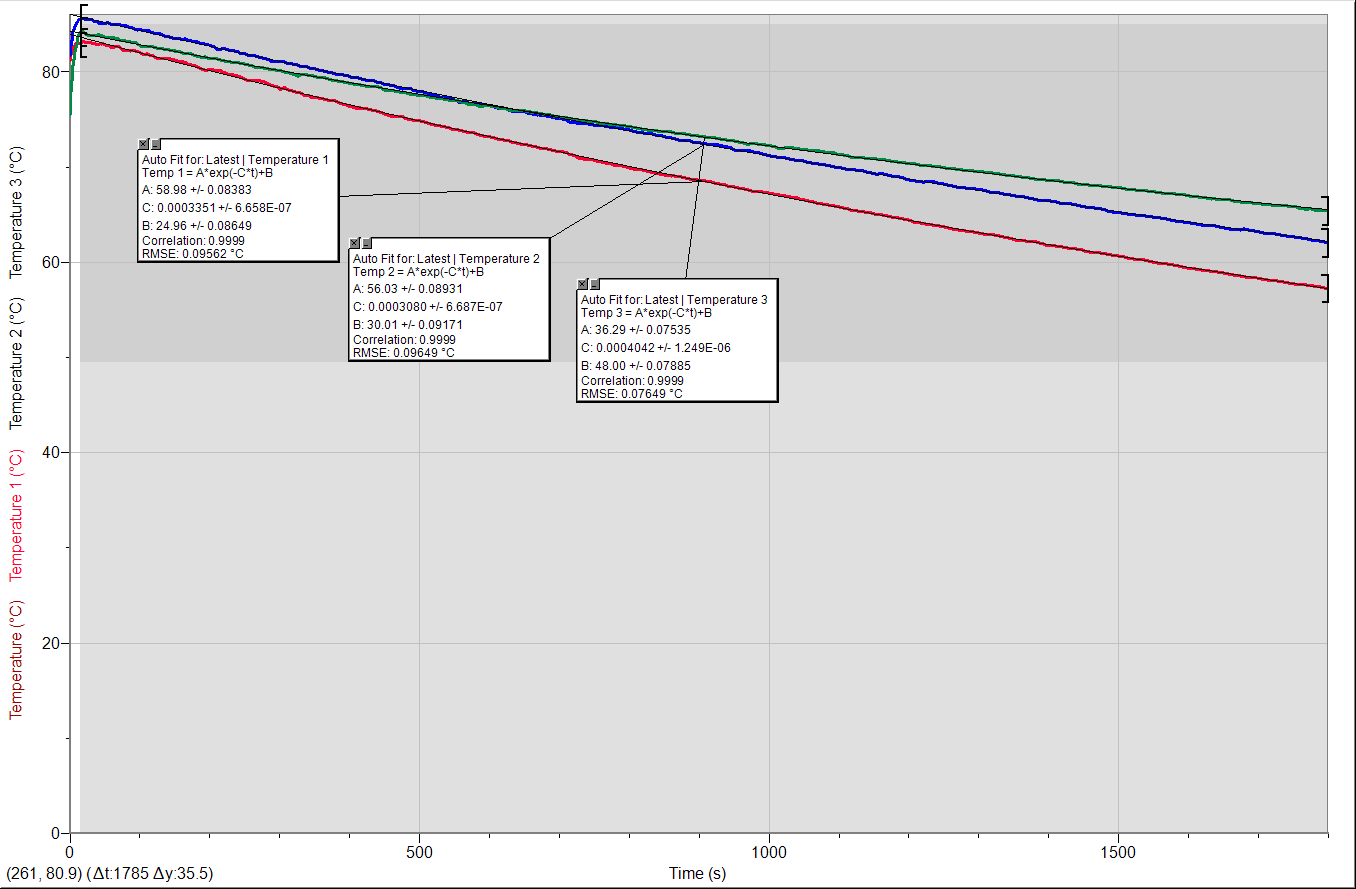
\includegraphics[width=0.4\textwidth]{insulated.png}
            \end{center}
        \end{mdframed}
    \end{enumerate}

    \pagebreak

    \section*{Conclusions}

    \subsection*{Part 1: Convective Cooling}

    \begin{enumerate}
        \item [4.]\mbox{}
        \begin{mdframed}
            The further away the thermos was, the slower the water in the thermos lost heat.
        \end{mdframed}

        \item [5.]\mbox{}
        \begin{mdframed}
            \begin{equation}
                \begin{gathered}
                \frac{0.001341}{0.000854} = 1.57
                \end{gathered}
            \end{equation}

            The 10cm thermos is cooling at a factor of 1.57 times faster than the 100cm thermos.
        \end{mdframed}

        \item [6.]\mbox{}
        \begin{mdframed}
            The thermometer would read -20$^{\circ}$F. The wind siphons energy away from you, making it feel colder, but it's simply the rate of heat loss that's increased, making it feel colder, but it plays no role in the reading as the wind does not change the temperature of the air. If you were moving with the wind, the temperature would still say -20$^{\circ}$F, and if you moved in the opposite direction, the temperature would still read -20$^{\circ}$F.
        \end{mdframed}
    \end{enumerate}

    \subsection*{Part 2: Insulated Cooling}

    \begin{enumerate}
        \item [7.]\mbox{}
        \begin{mdframed}
            The water lost energy by conduction as there was no material taking away heat; it was transferring its heat into the environment.
        \end{mdframed}

        \item [8.]\mbox{}
        \begin{mdframed}
            \begin{equation}
                \begin{gathered}
                \frac{0.004042}{0.0003351} = 12.06
                \end{gathered}
            \end{equation}

            The uninsulated container is cooling at a factor of 12.06 times faster than the heavily insulated container.
        \end{mdframed}

        \item [9.]\mbox{}
        \begin{mdframed}
            The down jacket simply adds more mass to the container walls, which decreases the rate of heat transfer. The vacuum removes as much material as possible, leaving a gap of very little material between the outside and the container which drastically reduces the rate of heat loss.
        \end{mdframed}        
    \end{enumerate}

    \pagebreak

    \subsection*{Part 3: Equilibrium Temperature}

    \begin{enumerate}
        \item [10.]\mbox{}
        \begin{mdframed}
            The equilibrium temperature would not change in either case; changing how fast the energy is transferred to the metal does not change the temperature at which no more energy is transferred.
        \end{mdframed}

        \item [11.]\mbox{}
        \begin{mdframed}
            \begin{center}
                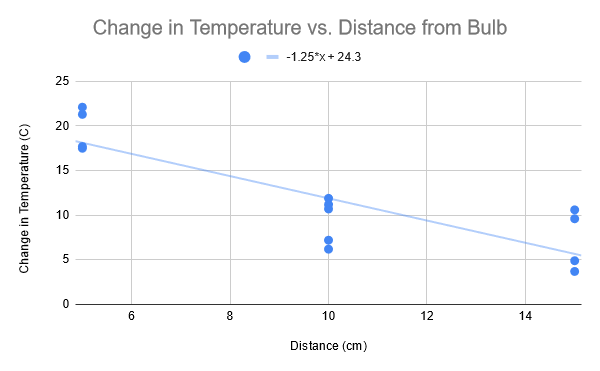
\includegraphics[width=0.8\textwidth]{q11-2.png}

                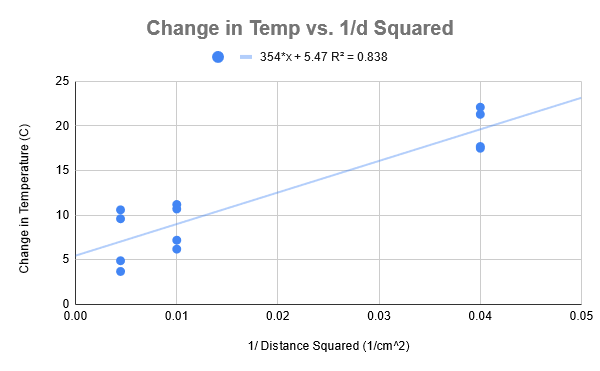
\includegraphics[width=0.8\textwidth]{q11.png}
            \end{center}
        \end{mdframed}

        \item [12.]\mbox{}
        \begin{mdframed}
            No; the temperature change varies inversely with the distance from the bulb. Inversing it to $\frac{1}{d^2}$ will result in a positive correlation between the two.
        \end{mdframed}
        
        \pagebreak

        \item [13.]\mbox{}
        \begin{mdframed}
            Compared to the graphs produced before, a bulb placed 30cm from the bulb would reach approximately $-1.25(30)+24.3 = -13.2^{\circ}$C, which would imply that 30cm would have little to no change in its temperature.
        \end{mdframed}
    \end{enumerate}
    
    \section*{General Questions}

    \begin{enumerate}
        \item [14.]\mbox{}
        \begin{mdframed}
            Earth's atmosphere's equilibrium temperature is increased by radiation from the sun.
        \end{mdframed}

        \item [15.]\mbox{}
        \begin{mdframed}
            All three share an area ($A$) variable.
            
            All three have a specific constant ($k$: thermal conductivity, $h$: conductive heat transfer coefficient, $\sigma$: Stefan-Boltzmann constant).

            All three share some form of heat/temperature variable.
        \end{mdframed}

        \item [16.]\mbox{}
        \begin{mdframed}
            Radiation: The sun heats the planet via radiation.

            Conduction: The coils on the top of a conduction stove.

            Convection: The air being circulated inside of a convection oven.
        \end{mdframed}

        \item [17.]\mbox{}
        \begin{mdframed}
            Snow is probably good at scattering visible radiation as it's white in color.

            Snow is probably bad at scattering infrared as blowtorches are effective at melting snow.
        \end{mdframed}

        \item [18.]\mbox{}
        \begin{mdframed}
            Insulating layers must be heated up first before their energy can be pulled either inside or outside of the window. The more layers there are, the longer it takes for heat to transfer through the window.
        \end{mdframed}

        \item [19.]\mbox{}
        \begin{mdframed}
            Both systems are not closed; they have an external force that's adding or removing energy. The airflow removes energy from the first and second experiments, and the outlet provides electrical energy that's converted to heat in the third experiment.
        \end{mdframed}
    \end{enumerate}
\end{document}